\chapter{Análisis de Resultados}
\label{chap:analisis}

\observacion{Poner descripción al nombre de las pruebas, por ejemplo no objetiva
    o subjetiva}
\observacion{Juntar cap análisis y resultados}
\observacion{Borrar los nos}
\observacion{Ver lo de aleatoriedad (variable) en subjetiva}

En este capítulo se muestran los resultados obtenidos en cada una de las pruebas 
y encuestas descriptas en el capítulo anterior. Los valores obtenidos son expuestos en
distintos formatos para mejorar su interpretación.

En la primera parte se describen los resultados obtenidos de la \emph{Prueba de interfaz de usuario} 
los cuales revelan los aspectos que debieron ser mejorados durante el desarrollo de 
la solución. 

En la segunda parte, se muestran los resultados obtenidos de la 
\emph{Encuesta de ubicación} los cuales muestran el porcentaje de alumnos que cumplen 
con los requisitos para formar parte del grupo de evaluación de la solución.

En la tercera parte, se muestran los resultados obtenidos de la \emph{Encuesta subjetiva} 
en donde se muestran las fortalezas y debilidades de la solución así como datos que miden 
la aceptación de la solución por parte del usuario. 

En la cuarta parte, se muestran los resultados obtenidos de la \emph{Encuesta objetiva} 
en donde se muestra el rendimiento de los alumnos en cuanto a preguntas relacionadas a 
los procedimientos simulados, tanto de los que forman parte de la muestra como de los que 
forman parte del grupo de control. Sin embargo, la diferencia de rendimientos entre 
estos dos grupos no pueden ser considerada como absoluta ya que no se considera que 
la cantidad de partidas que fueron jugadas por los usuarios sean suficientes para 
influenciar notablemente en su rendimiento.

En la quinta parte, se muestran los resultados obtenidos del \emph{Registro de actividades} 
en donde se muestra el desempeño de los usuarios en cada una de las partidas jugadas, así como 
el grado de uso de la solución, entre otros aspectos importantes.

Finalmente, en la sexta parte, se muestran las relaciones entre los resultados obtenidos en 
la \emph{Encuesta objetiva} y el \emph{Registro de actividades}.


%! TEX root = ../main.tex
\section{Interfaz de Usuario}
\label{sec:res_interfaz}
\observacion{Pruebas preliminares de usabilidad}

En la sección~\ref{sec:interfaz} se describe la prueba de interfaz realizada
durante el desarrollo de \fixme{la solución}{de la UI}, a fin de validar las
hipótesis asumidas y evaluar la usabilidad de la solución.

Esta prueba se divide en dos partes, en la primera, denominada
\emph{Simulación}, los sujetos de prueba utilizan la aplicación, y en la
segunda parte, denominada \emph{Encuesta}, los mismos completan una encuesta
sobre su apreciación de la solución.

\subsection{Simulación}

Las grabaciones realizadas a las sesiones de los usuarios se utilizan para medir
el grado de facilidad de aprendizaje de la interfaz de usuario.

Dados los tres grupo descriptos en~\ref{sec:evaluacion_interfaz_variables}, la
tabla~\ref{tab:interfaz_tiempo_acciones} \fixme{muestra}{tiempo} el tiempo, en segundos,
que le tomo a cada usuario realizar cada una de las acciones la primera vez y
el tiempo que les tomo en promedio las demás veces, para cada una de los grupos
de acciones.

\observacion{Hacer énfasis en la comparación entre el primer y los siguientes}

\begin{table}[!hbt]
\centering
\begin{tabular}{|c|c|c|c|c|c|c|}
\hline
\rowcolor{gris} \textbf{} & \multicolumn{2}{|c|}{\textbf{Menú Contextual}} &
\multicolumn{2}{|c|}{\textbf{Menú de la Interfaz}} &
\multicolumn{2}{|c|}{\textbf{Herramienta}}\\
\hline
\rowcolor{gris} Usuario & Primera & Siguientes & Primera & Siguientes & Primera & Siguientes \\
\hline 1 &  8 &  2.25 &  3 & 9.14 & 11 & 3.0 \\
\hline 2 & 30 &  7.00 &  4 & 3.57 &  7 & 4.5 \\
\hline 3 &  5 &  2.25 &  5 & 1.86 &  1 & 1.0 \\
\hline 4 &  2 & 13.00 &  4 & 2.00 &  1 & 0.5 \\
\hline 5 & 18 &  2.75 &  6 & 4.43 &  6 & 3.0 \\
\hline 6 &  4 & 14.25 & 11 & 7.86 & 13 & 4.0 \\
\hline 7 &  5 &  8.00 &  4 & 4.71 & 20 & 2.5 \\
\hline 8 &  3 &  2.33 & 10 & 3.57 &  3 & 6.5 \\
\hline
\textbf{Promedio} & 9.38 & 6.37 & 5.88 & 4.64 & 7.75 & 3.125 \\
\end{tabular}
\caption{Tiempo por acciones la primera vez y las siguientes veces que se realizo}
\label{tab:interfaz_tiempo_acciones}
\end{table}

En la tabla~\ref{tab:interfaz_tiempo_acciones} se observa consistentemente una
\fixme{mejora}{En relación a qué?} en el tiempo de realización de una acción con
respecto a la primera vez que es realizada. 

\begin{figure}[hbt!]
\centering
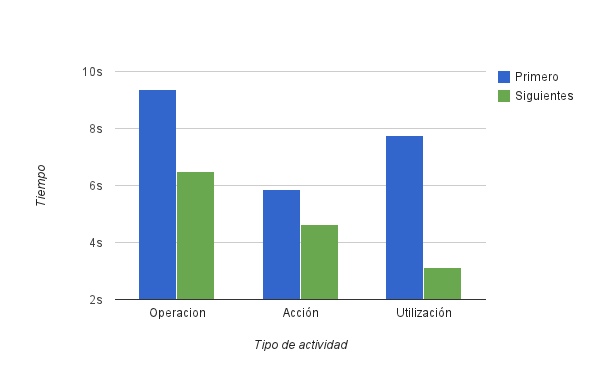
\includegraphics[width=14cm]{resultados/imagenes/interfaz_tiempo_actividades.png}
\caption{Tiempo por tipo de actividad}
\label{fig:interfaz_tiempo_acciones}
\end{figure}

En la figura~\ref{fig:interfaz_tiempo_acciones} se observa como en promedio el
usuario aprende, y en las siguientes acciones similares demora menos tiempo,
este es un factor importante y es el objetivo de esta prueba pues muestra que la
interfaz es fácil de usar, y con tres movimientos básicos, el usuario puede
utilizarla sin mayores inconvenientes. Se observa una mejoría del $30\%$ en las
acciones \emph{Menú Contextual}, $21\%$ en las acciones de tipo \emph{Menú de la
    Interfaz} y finalmente, una mejoría del $60\%$ en las acciones de tipo
\emph{Herramienta}.


La tabla~\ref{tab:interfaz_cantidad_espaciales} nos muestra la cantidad de
movimientos espaciales realizados por los usuarios, se observa que en promedio
se desplazaron $10,88$ veces por el escenario, y $6,75$ veces acercaron o
alejaron la cámara del paciente.

\observacion{Hay que dejar bien en claro de donde sale esto, por que es
importante entender el significado de esta diferencia}

\begin{table}[H]
\centering
\begin{tabular}{lrrr}
\toprule
\textbf{Jugador}  & \textbf{Movimiento} & \textbf{Zoom} & \textbf{Total} \\
\midrule
1        & 18         & 2    & 20 \\
2        & 7          & 8    & 15 \\
3        & 14         & 12   & 26 \\
4        & 9          & 14   & 23 \\
5        & 5          & 8    & 13 \\
6        & 14         & 4    & 18 \\
7        & 16         & 3    & 19 \\
8        & 4          & 3    &  7 \\
\midrule
\textbf{Promedio} & \textbf{10,88}      & \textbf{6,75} & \textbf{17,63} \\
\bottomrule
\end{tabular}
\caption{Cantidad de movimientos espaciales}
\label{tab:interfaz_cantidad_espaciales}
\end{table}

No existe una cantidad mínima o máxima que el usuario debería acercar o mover la
cámara, en cambio, los datos mostrados en~\ref{tab:interfaz_cantidad_espaciales},
muestran que no son necesarias demasiadas acciones, juntando esta información,
con la información proveída en la tabla~\ref{tab:interfaz_tiempo_total}, se ve
que en promedio los usuarios realizaron $1,7$ movimientos por minuto.

\begin{table}[!hbt]
\centering
\begin{tabular}{lrrr}
\toprule
\textbf{Alumno} & \textbf{Tiempo} \\
\midrule
1        & 8:32 \\
2        & 6:03 \\
3        & 8:33 \\
4        & 5:17 \\
5        & 6:55 \\
6        & 8:40 \\
7        & 7:03 \\
8        & 10:27 \\
\midrule
\textbf{Promedio} & \textbf{7:41} \\
\bottomrule
\end{tabular}
\caption{Tiempo de prueba por usuario}
\label{tab:interfaz_tiempo_total}
\end{table}

El tiempo total que se observa en la tabla~\ref{tab:interfaz_tiempo_total},
muestra que en promedio a cada alumno le tomo $7:41$ minutos realizar todos los
pasos especificados, es importante notar que este tiempo incluye el tiempo de
adaptación. 



\begin{table}[!hbt]
\centering
\begin{tabular}{lrrr}
\toprule
\textbf{Alumno} & \textbf{Pasos requeridos} \\
\midrule
1 & 19 \\
2 & 15 \\
3 & 18 \\
4 & 15 \\
5 & 18 \\
6 & 16 \\
7 & 19 \\
8 & 14 \\
\midrule
\textbf{Promedio} & \textbf{16,75} \\
\bottomrule
\end{tabular}
\caption{Acciones realizadas por usuario}
\label{tab:interfaz_acciones}
\end{table}

La tabla~\ref{tab:interfaz_acciones} nos muestra la cantidad de acciones que
realizaron los alumnos, junto con las acciones correctas para llevar a cabo el
procedimiento. Se observa que en promedio realizaron $16.75$ acciones correctas,
esto permite identificar en que parte de procedimiento los usuarios tienen
inconvenientes en cuanto al uso de la interfaz.

\subsection{Encuesta}

\fixme{Como fue descripta en la sección~\ref{sec:interfaz} la encuesta es
realizada a cada usuario}{Mejorar}, y es utilizada para obtener el grado de
disconformidad de los mismos. Se utiliza la disconformidad para resaltar los
puntos débiles, y así, aquellas variables que tengan el mayor porcentaje serán
las que deben ser arregladas.

Las preguntas que forman parte de la  encuesta son agrupadas en cuanto a
aspectos de calidad gráfica, interacción con el entorno, interacción con los
objetos, características del entorno, usabilidad de la interfaz e integración
con el hardware.

Luego de estas agrupaciones obtenemos el resultado que se muestra en la
tabla~\ref{tab:interfaz_disconformidad_metrica}. En esta tabla se puede observar
que las mayores disconformidades son con respecto a la usabilidad de la interfaz
que llega al $51\%$, la interacción de los usuarios con el entorno que llega al
$50\%$, la interacción con los objetos que llega al $49\%$. Luego, se pueden
observar también otras disconformidades con menor porcentaje, las
características del entorno con un  $33\%$, la integración con el hardware con
un  $27\%$ y por ultimo, la calidad gráfica con un  $17\%$.

\observacion{Hay que explicar que estas pruebas se hicieron de forma previa a
las demás y que se arreglan algunos casos}

\begin{table}[H]
\centering
\begin{tabular}{lr}
\toprule
Métrica & Disconformidad \\
\midrule
Calidad Gráfica         & 0.17 \\
Interacción Entorno     & 0.50\\
Interacción Objetos     & 0.49\\
Características Entorno & 0.33\\
Usabililidad Interfaz   & 0.51\\
Integración Hardware    & 0.27\\
\bottomrule
\end{tabular}
\caption{Disconformidad por métrica}
\label{tab:interfaz_disconformidad_metrica}
\end{table}

La conclusión de esta prueba de interfaz, es que si bien, pudo ser utilizada sin
mayores inconvenientes, existe un alto grado de disconformidad con la interfaz,
además cabe resaltar, los sujetos de prueba son personas acostumbradas al uso de
tecnologías similares. Otros puntos débiles encontrados en esta prueba son la
interacción con el entorno y  con los objetos.

Como resultado de esta prueba, la interfaz y la interacción con objetos y
elementos sufren modificaciones a fin de su utilización con usuarios no
técnicos.

Las demás pruebas mencionadas en este capítulo son realizadas con la versión
final de la solución, la cual es obtenida luego de las mejoras realizadas a los
puntos débiles detectados por esta prueba.

%! TEX root = ../main.tex


\section{Encuesta de Ubicación}
\label{sec:res_UBICACION}

Como se indicó en la sección~\ref{sec:ubicacion}, se agrupa a los alumnos
encuestados de acuerdo a las características de sus dispositivos móviles y del
acceso a internet.

En la figura~\ref{fig:ubicacion_acceso_internet} se puede observar que de 93
encuestados, el $94,6\%$ tiene acceso a internet al menos en algún momento y que
solo el $5.4\%$ no tiene acceso a internet en sus dispositivos móviles.

\begin{figure}[ht!]
\centering
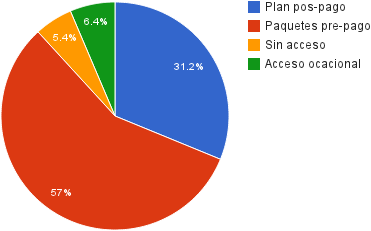
\includegraphics[scale=0.8]{resultados/imagenes/ubicacion_acceso_internet.png}
\caption{Acceso a internet desde dispositivos móviles}
\label{fig:ubicacion_acceso_internet}
\observacion{no habia otras caracteristicas}
\end{figure}

Por otro lado, en la figura\ref{fig:ubicacion_sistemas_operativos} se muestra
los sistemas operativos móviles utilizados por los usuarios encuestados. Se
puede observar que Android lidera con un $61.3\%$, le sigue Windows Phone con un
$12.9\%$.

\begin{figure}[ht!]
\centering
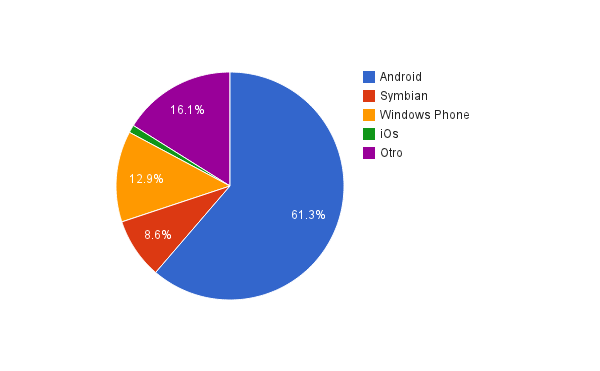
\includegraphics[scale=0.8]{resultados/imagenes/ubicacion_sistemas_operativos.png}
\caption{Sistemas operativos móviles utilizados}
\label{fig:ubicacion_sistemas_operativos}
\observacion{Meter a la par de otros}
\end{figure}

Por último, se discrimina a los encuestados para determinar cuantos de ellos
tiene dispositivos móviles que cumplen los requisitos mínimos para utilizar la
solución propuesta según lo descrito en la sección~\ref{sec:ubicacion}. En la
figura~\ref{fig:ubicacion_requisitos_minimos} se puede observar que el $18,3\%$
de los encuestados cumplen con los requisitos.

\begin{figure}[ht!]
\centering
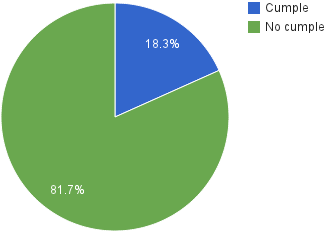
\includegraphics[scale=0.8]{resultados/imagenes/ubicacion_requisitos_minimos.png}
\caption{Dispositivos que cumplen con los requisitos mínimos para la prueba}
\label{fig:ubicacion_requisitos_minimos}
\observacion{Que conclusiones podría quitar de esto?}
\end{figure}

\observacion{Acercar más los gráficos}

%! TEX root = ../main.tex

\section{Encuesta Subjetiva}

En el análisis de los resultados de las encuestas subjetivas, existieron alumnos
que no respondieron todas las preguntas, para tratar este tipo de casos, es
importante analizar la naturaleza del patrón de datos
faltantes\cite{carpita2011imputation}. 

La información recogida por la encuesta muestra que hay datos faltantes, como se
explico en~\ref{sec:informacion_faltante}, esta información faltante es
completamente aleatoria en relación a la variable medida y a las demás
variables, de hecho, una sola encuesta tiene información faltante, así, se
establece que el tipo de información faltante es \emph{Información faltante
    completamente aleatoria}.

En su resumen de las diferentes técnicas y cuando se deben utilizar,
\cite{tsikriktsis2005review}, recomienda la utilización de la sustitución basada
en promedio por caso. Así, se completan los valores faltantes con el promedio de
respuestas completadas por el usuario.

\subsection{Resultados}

Se presentan a continuación los resultados de las encuestas, agrupados por los
factores definidos en~\ref{sec:variables}.

La tabla~\ref{tab:subjetiva_conformidad_exploracion} nos muestra las respuestas
de los alumnos a las preguntas relacionadas al factor exploración, son cuatro
preguntas, las cuales fueron descritas en~\ref{sec:sub_exploracion}. 

\begin{table}[!hbt]
\centering
\begin{tabular}{@{} *{5}{r} @{}}
\toprule
& \multicolumn{4}{c}{Exploración} \\
\cmidrule(lr){2-5}
Alumno &
\parbox{3cm}{Funciones realizadas por los elementos del juego} &
\parbox{3cm}{Aleatoriedad para afianzar conocimientos} &
\parbox{2.5cm}{Aleatoriedad para representar realismo} &
\parbox{2.5cm}{Facilidad de uso}  \\
\midrule
1         & 2   & 6   & 5   & 6  \\
2         & 6   & 6   & 4   & 6  \\
3         & 3   & 3   & 5   & 5  \\
4         & 6   & 6   & 6   & 6  \\
5         & 6   & 6   & 2   & 5  \\
6         & 6   & 6   & 6   & 6  \\
7         & 7   & 7   & 7   & 7  \\
8         & 6   & 6   & 7   & 7  \\
9         & 5   & 7   & 7   & 7  \\
10        & 6   & 7   & 6   & 6  \\
11        & 7   & 6   & 7   & 6  \\
\bottomrule
\end{tabular}
\caption{Resultados de la encuesta subjetiva relacionados al factor Exploración}
\label{tab:subjetiva_conformidad_exploracion}
\end{table}

La tabla~\ref{tab:subjetiva_conformidad_gamificacion} muestra las respuestas de
los alumnos a las preguntas relacionadas al factor \textit{Gamificación}, son
cinco preguntas, las cuales fueron descritas en~\ref{sec:sub_gamificacion}. 

\begin{table}[!hbt]
\centering
\begin{tabular}{@{} *{5}{r} @{}}
\toprule
& \multicolumn{4}{c}{Gamificación} \\
\cmidrule(lr){2-5}
Alumno &
\parbox{2.5cm}{Motivación del puntaje} &
\parbox{2.5cm}{Importancia del puntaje} &
\parbox{3cm}{Socialización de los puntajes} &
\parbox{3cm}{Medición del tiempo como motivación} \\
\midrule
1  & 6 & 4 & 4 & 7  \\
2  & 7 & 4 & 6 & 6  \\
3  & 6 & 6 & 5 & 6  \\
4  & 1 & 4 & 6 & 1  \\
5  & 2 & 2 & 7 & 7  \\
6  & 6 & 5 & 4 & 6  \\
7  & 7 & 7 & 6 & 7  \\
8  & 7 & 7 & 7 & 7  \\
9  & 7 & 7 & 7 & 7  \\
10 & 7 & 4 & 5 & 7  \\
11 & 5 & 4 & 5 & 6  \\
\bottomrule
\end{tabular}
\caption{Resultados de la encuesta subjetiva relacionados al factor Gamificación}
\label{tab:subjetiva_conformidad_gamificacion}
\end{table}

La tabla~\ref{tab:subjetiva_conformidad_inmersion} muestra las respuestas de
los alumnos a las preguntas relacionadas al factor \textit{Inmersión}, son
cinco preguntas, las cuales fueron descritas en~\ref{sec:sub_inmersion}. 

\begin{table}[!hbt]
\centering
\begin{tabular}{@{} *{6}{r} @{}}
\toprule
& \multicolumn{5}{c}{Inmersión} \\
\cmidrule(lr){2-6}
Alumno &
\parbox{2.5cm}{Escenografía para entrar en ambiente} &
\parbox{2.5cm}{Juegos cortos como ayuda para la repetición} &
\parbox{2.5cm}{Gráficos en tres dimensiones para entender el entorno} &
\parbox{2.5cm}{Realismo a través de ordenes verbales} &
\parbox{2.5cm}{Simulación como herramienta} \\
\midrule
1  & 4 & 6 & 4 & 5 & 3  \\
2  & 6 & 6 & 6 & 6 & 6  \\
3  & 6 & 6 & 6 & 5 & 6  \\
4  & 4 & 6 & 7 & 5 & 6  \\
5  & 6 & 6 & 5 & 6 & 6  \\
6  & 6 & 6 & 6 & 4 & 4  \\
7  & 7 & 7 & 7 & 7 & 7  \\
8  & 6 & 7 & 7 & 7 & 7  \\
9  & 6 & 7 & 7 & 7 & 7  \\
10 & 6 & 3 & 4 & 6 & 6  \\
11 & 5 & 3 & 5 & 5 & 4  \\
\bottomrule
\end{tabular}
\caption{Resultados de la encuesta subjetiva relacionados al factor Inmersión}
\label{tab:subjetiva_conformidad_inmersion}
\end{table}


La tabla~\ref{tab:subjetiva_conformidad_pedagogia} agrupa las respuestas de los
alumnos según el factor pedagógico, son tres preguntas, las cuales fueron
descritas en~\ref{sec:sub_pedagogia}. 

\begin{table}[!hbt]
\centering
\begin{tabular}{@{} *{4}{r} @{}}
\toprule
& \multicolumn{3}{c}{Pedagogía} \\
\cmidrule(lr){2-4}
Alumno &
\parbox{4cm}{La solución para memorizar y comprender el procedimiento} &
\parbox{4cm}{Falta de pistas como ayuda al aprendizaje} &
\parbox{4cm}{Suficiencia de los botones que indican acciones} \\
\midrule
1  & 6 & 6 & 6  \\
2  & 6 & 6 & 7  \\
3  & 4 & 6 & 6  \\
4  & 6 & 7 & 6  \\
5  & 7 & 5 & 6  \\
6  & 4 & 4 & 6  \\
7  & 7 & 6 & 7  \\
8  & 6 & 7 & 7  \\
9  & 7 & 7 & 7  \\
10 & 6 & 7 & 7  \\
11 & 5 & 6 & 5  \\
\bottomrule
\end{tabular}
\caption{Resultados de la encuesta subjetiva relacionados al factor Pedagogía}
\label{tab:subjetiva_conformidad_pedagogia}
\end{table}


La tabla~\ref{tab:subjetiva_conformidad_representacion} agrupa las respuestas de
los alumnos según la calidad de presentación, son cinco preguntas, las cuales
fueron descritas en~\ref{sec:sub_representacion}. 

\begin{table}[!hbt]
\centering
\begin{tabular}{@{} *{6}{r} @{}}
\toprule
& \multicolumn{5}{c}{Representación} \\
\cmidrule(lr){2-6}
Alumno &
\parbox{2.5cm}{Movimientos motrices del paciente} &
\parbox{2.5cm}{Movimientos oculares del paciente} &
\parbox{2.5cm}{Reacción verbal del paciente} &
\parbox{2.5cm}{Distinción entre los estados del paciente} &
\parbox{2.5cm}{Acciones las herramientas} \\
\midrule
1  & 6 & 6 & 2 & 5 & 2  \\
2  & 4 & 5 & 5 & 6 & 4  \\
3  & 5 & 3 & 3 & 3 & 3  \\
4  & 6 & 5 & 2 & 4 & 2  \\
5  & 2 & 2 & 6 & 6 & 6  \\
6  & 6 & 4 & 6 & 6 & 6  \\
7  & 7 & 6 & 5 & 7 & 5  \\
8  & 6 & 7 & 7 & 7 & 5  \\
9  & 5 & 6 & 2 & 7 & 6  \\
10 & 6 & 4 & 4 & 4 & 5  \\
11 & 6 & 4 & 6 & 6 & 5  \\
\bottomrule
\end{tabular}
\caption{Resultados de la encuesta subjetiva relacionados al factor
    Representación}
\label{tab:subjetiva_conformidad_representacion}
\end{table}


La tabla~\ref{tab:subjetiva_conformidad_retroalimentacion} agrupa las respuestas
de los alumnos según la calidad de retroalimentación, son tres preguntas, las
cuales fueron descritas en~\ref{sec:sub_retroalimentacion}. 

\begin{table}[!hbt]
\centering
\begin{tabular}{@{} *{4}{r} @{}}
\toprule
& \multicolumn{3}{c}{Retroalimentación} \\
\cmidrule(lr){2-4}
Alumno &
\parbox{4cm}{Detalles de los pasos realizados incorrectamente} &
\parbox{4cm}{Suficiencia de los detalles de los pasos realizados incorrectamente} &
\parbox{4cm}{Iconos para representar el estado del jugador} \\
\midrule
1  & 3 & 2 & 7  \\
2  & 5 & 4 & 6  \\
3  & 3 & 6 & 6  \\
4  & 6 & 6 & 6  \\
5  & 6 & 1 & 6  \\
6  & 2 & 6 & 6  \\
7  & 6 & 7 & 7  \\
8  & 6 & 6 & 7  \\
9  & 6 & 6 & 7  \\
10 & 5 & 4 & 6  \\
11 & 4 & 5 & 6  \\
\bottomrule
\end{tabular}
\caption{Resultados de la encuesta subjetiva relacionados al factor
    Retroalimentación}
\label{tab:subjetiva_conformidad_retroalimentacion}
\end{table}


La tabla~\ref{tab:subjetiva_conformidad_utilidad} agrupa las respuestas de los
alumnos según la utilidad de la solución, son tres preguntas, las cuales fueron
descritas en~\ref{sec:sub_utilidad}. 


\begin{table}[!hbt]
\centering
\begin{tabular}{@{} *{6}{r} @{}}
\toprule
& \multicolumn{3}{c}{Utilidad} \\
\cmidrule(lr){2-4}
Alumno &
\parbox{4cm}{Simulación para complementar el estudio en clase y laboratorio} &
\parbox{4cm}{Simulación provee más facilidades para el estudio} &
\parbox{4cm}{Interacción con el paciente} \\
\midrule
1  & 7 & 5 & 7  \\
2  & 6 & 6 & 6  \\
3  & 6 & 6 & 6  \\
4  & 2 & 6 & 6  \\
5  & 2 & 6 & 6  \\
6  & 6 & 6 & 6  \\
7  & 7 & 6 & 7  \\
8  & 5 & 6 & 7  \\
9  & 7 & 7 & 7  \\
10 & 1 & 7 & 7  \\
11 & 6 & 4 & 5  \\
\bottomrule
\end{tabular}
\caption{Resultados de la encuesta subjetiva relacionados al factor Utilidad}
\label{tab:subjetiva_conformidad_utilidad}
\end{table}

\section{Agrupamiento de datos}

Los resultados se resumen en la tabla~\ref{tab:subjetiva_conformidad_resumen},
se muestra el número de alumno para identificar a un alumno y el promedio de sus
respuestas en la encuesta, se muestra el promedio de las mismas.

\begin{table}[!hbt]
\begin{tabular}{llllllllr}
\toprule
\textbf{\shortstack{Número de \\alumno}}         &
\begin{sideways}\textbf{Gamificación}                    \end{sideways}        &
\begin{sideways}\textbf{Exploración}                     \end{sideways}        &
\begin{sideways}\textbf{Inmersión}                       \end{sideways}        &
\begin{sideways}\textbf{Pedagogía}                       \end{sideways}        &
\begin{sideways}\textbf{Representación}                  \end{sideways}        &
\begin{sideways}\textbf{Retroalimentación}               \end{sideways}        &
\begin{sideways}\textbf{Utilidad}                        \end{sideways}        &
\textbf{\shortstack{Promedio\\de respuestas}}\\
\midrule
1              & 5 & 5 & 4 & 6 & 4 & 4 & 6 & 5 \\
2              & 6 & 6 & 6 & 6 & 5 & 5 & 6 & 6 \\
3              & 4 & 6 & 6 & 5 & 3 & 5 & 6 & 5 \\
4              & 6 & 3 & 6 & 6 & 4 & 6 & 5 & 5 \\
5              & 5 & 5 & 6 & 6 & 4 & 4 & 5 & 5 \\
6              & 6 & 5 & 5 & 5 & 6 & 5 & 6 & 5 \\
7              & 7 & 7 & 7 & 7 & 6 & 7 & 7 & 7 \\
8              & 7 & 7 & 7 & 7 & 6 & 6 & 6 & 7 \\
9              & 7 & 7 & 7 & 7 & 5 & 6 & 7 & 6 \\
10             & 6 & 6 & 5 & 7 & 5 & 5 & 5 & 5 \\
11             & 7 & 5 & 4 & 5 & 5 & 5 & 5 & 5 \\
\midrule
Promedio Total & 6 & 6 & 6 & 6 & 5 & 5 & 6 & 6 \\
\bottomrule
\end{tabular}
\caption{Resultados de la encuesta subjetiva}
\label{tab:subjetiva_conformidad_resumen}
\end{table}

Se observa que el el puntaje más bajo en el promedio final es 5 que significa
\textit{Parcialmente de acuerdo}, y el más alto es 7, que significa
\textit{Totalmente de acuerdo}, se observa además el puntaje 6, que significa
\textit{De acuerdo}. 


Como se explica en la sección~\ref{sec:likert}, estos resultados están sujetos a
tendencias, para ello se aplica el método de doble
estandarización\cite{Pagolu2011}.

Con el resultado final de la estandarización diferenciamos cuales son los puntos
fuertes y cuales los puntos débiles de la solución propuesta con respecto a las
respuestas dadas por los usuarios. Estos valores son relativos a las respuestas
originales dadas en la encuesta, los resultados se muestran en la
tabla~\ref{tab:subjetiva_conformidad_corregida}.

\begin{table}[!hbt]
\centering
\begin{tabular}{lrrrrrrrr}
\toprule
\textbf{\shortstack{Número de \\alumno}}                                &
\begin{sideways}\textbf{Gamificación}                    \end{sideways} &
\begin{sideways}\textbf{Exploración}                     \end{sideways} &
\begin{sideways}\textbf{Inmersión}                       \end{sideways} &
\begin{sideways}\textbf{Pedagogía}                       \end{sideways} &
\begin{sideways}\textbf{Representación}                  \end{sideways} &
\begin{sideways}\textbf{Retroalimentación}               \end{sideways} &
\begin{sideways}\textbf{Utilidad}                        \end{sideways} &
\textbf{\shortstack{Promedio\\de respuestas}}\\
\midrule
1              & 0.45 & 0.55 & 0.20 & 0.63 & 0.44 & 0.41 & 0.82 & 0.47 \\
2              & 0.33 & 0.53 & 0.49 & 0.61 & 0.27 & 0.13 & 0.52 & 0.41 \\
3              & 0.17 & 0.86 & 0.87 & 0.67 & 0.13 & 0.67 & 1.00 & 0.60 \\
4              & 0.75 & 0.31 & 0.63 & 0.81 & 0.47 & 0.78 & 0.54 & 0.59 \\
5              & 0.46 & 0.58 & 0.69 & 0.67 & 0.57 & 0.50 & 0.54 & 0.58 \\
6              & 1.00 & 0.73 & 0.68 & 0.42 & 0.90 & 0.67 & 1.00 & 0.78 \\
7              & 1.00 & 0.79 & 1.00 & 0.67 & 0.50 & 0.87 & 0.78 & 0.80 \\
8              & 0.75 & 1.00 & 0.83 & 0.75 & 0.70 & 0.70 & 0.44 & 0.75 \\
9              & 0.90 & 1.00 & 0.93 & 1.00 & 0.64 & 0.92 & 1.00 & 0.90 \\
10             & 0.79 & 0.74 & 0.54 & 0.92 & 0.60 & 0.60 & 0.67 & 0.68 \\
11             & 0.75 & 0.42 & 0.08 & 0.25 & 0.60 & 0.35 & 0.25 & 0.39 \\
\midrule
\textbf{Promedio Total} & 0.67 & 0.68 & 0.63 & 0.67 & 0.53 & 0.60 & 0.69 & 0.63 \\
\bottomrule
\end{tabular}
\caption{Resultados de la encuesta subjetiva con doble estandarización}
\label{tab:subjetiva_conformidad_corregida}
\end{table}

Para obtener una mejor visión de las fortalezas y debilidades de la solución
propuesta, se presenta el gráfico de kiviat~\ref{fig:subjetiva_kiviat}, en la
misma se puede observar cuales son los puntos débiles de la solución.

\begin{figure}[!ht]
\begin{tikzpicture}[label distance=.15cm]
\tkzKiviatDiagram[radial=2,
                    lattice=2, step=2,
                    scale=2.3]%
                {Gamificación,
                 Exploración,
                 Inmersión,
                 Pedagogía,
                 Representación,
                 Retroalimentación,
                 Utilidad}
\tkzKiviatLine[thick,
                color=blue,
                mark=ball,
                ball color=red,
                mark size=1pt,opacity=.2, 
                fill=red!20](0.67,0.68,0.63,0.67,0.53,0.60,0.69)
\end{tikzpicture}
\label{fig:subjetiva_kiviat}
\caption{Gráfico de Kiviat de los factores evaluados}
\end{figure}

En el gráfico se observa en la figura, que las principales debilidades de
la solución son la representación y la retroalimentación.

Es importante notar que los datos la figura~\ref{fig:subjetiva_kiviat}
y~\ref{tab:subjetiva_conformidad_corregida} son relativas a los datos de la
tabla~\ref{tab:subjetiva_conformidad_resumen}, es decir, que la representación
es el punto más débil, pero se ve en~\ref{tab:subjetiva_conformidad_resumen}
que el valor es 5 de 7, lo que indica que es un punto aceptable, y entre
los factores analizados es el que menos aprobación obtuvo.



\subsection{Correlacion}

En la tabla~\ref{tab:subjetiva_correlacion} se muestra la correlación entre los
factores analizados, las mismas fueron calculadas según lo explicado en la
sección \todox{Agregar sección de correlación}. En resumen se pueden notar las
siguientes correlaciones:

\begin{itemize}
\item \textbf{Gamification y Exploración, 0.33} Correlación positiva moderada.
\item \textbf{Gamification y Pedagogía, 0.27} Correlación positiva débil.
\item \textbf{Gamificatoin e Inmersión, 0.48} Correlación positiva fuerte.
\item \textbf{Gamification y Representación, 0.81} Correlación positiva muy fuerte.
\item \textbf{Gamification y Retroalimentación, 0.66} Correlación positiva fuerte.
\item \textbf{Gamification y Utilidad, 0.26} Correlación positiva débil.
\item \textbf{Exploración y Pedagogía, 0.52} Correlación positiva fuerte.
\item \textbf{Exploración e Inmersión, 0.53} Correlación positiva fuerte.
\item \textbf{Exploración y Representación, 0.44} Correlación positiva fuerte.
\item \textbf{Exploración y Retroalimentación, 0.37} Correlación positiva moderada.
\item \textbf{Exploración y Utilidad, 0.69} Correlación positiva fuerte.
\item \textbf{Pedagogía e Inmersión, 0.57} Correlación positiva fuerte.
\item \textbf{Pedagogía y Representación, 0.23} Correlación positiva débil.
\item \textbf{Pedagogía y Retroalimentación, 0.68} Correlación positiva fuerte.
\item \textbf{Pedagogía y Utilidad, 0.54} Correlación positiva fuerte.
\item \textbf{Inmersión y Representación, 0.39} Correlación positiva moderada.
\item \textbf{Inmersión y Retroalimentación, 0.49} Correlación positiva fuerte.
\item \textbf{Inmersión y Utilidad, 0.35} Correlación positiva moderada.
\item \textbf{Representación y Retroalimentación, 0.51} Correlación positiva fuerte.
\item \textbf{Representación y Utilidad, 0.36} Correlación positiva moderada.
\item \textbf{Retroalimentación y Utilidad, 0.52} Correlación positiva fuerte.
\end{itemize}

\begin{table}[!hbt]
\centering
\begin{tabular}{l|lllllllr}
\toprule
        &
\begin{sideways}\textbf{Gamificación}                    \end{sideways}        &
\begin{sideways}\textbf{Exploración}                     \end{sideways}        &
\begin{sideways}\textbf{Inmersión}                       \end{sideways}        &
\begin{sideways}\textbf{Pedagogía}                       \end{sideways}        &
\begin{sideways}\textbf{Representación}                  \end{sideways}        &
\begin{sideways}\textbf{Retroalimentación}               \end{sideways}        &
\begin{sideways}\textbf{Utilidad}                        \end{sideways}      \\
\midrule
\textbf{Gamification}      & 1    & 0.33 & 0.27 & 0.48 & 0.81 & 0.66  & 0.27 \\
\textbf{Exploración}       & 0.33 & 1    & 0.52 & 0.53 & 0.44 & 0.37  & 0.69 \\
\textbf{Inmersión}         & 0.27 & 0.52 & 1    & 0.57 & 0.23 & 0.68  & 0.54 \\
\textbf{Pedagogía}         & 0.48 & 0.53 & 0.57 & 1    & 0.39 & 0.49  & 0.35 \\
\textbf{Representación}    & 0.81 & 0.44 & 0.23 & 0.39 & 1    & 0.51  & 0.36 \\
\textbf{Retroalimentación} & 0.66 & 0.37 & 0.68 & 0.49 & 0.51 & 1     & 0.52 \\
\textbf{Utilidad}          & 0.27 & 0.69 & 0.54 & 0.35 & 0.36 & 0.52  & 1 \\
\bottomrule
\end{tabular}
\caption{Correlación entre los factores analizados} 
\label{tab:subjetiva_correlacion}
\end{table}

\section{Encuesta Objetiva}
\label{sec:res_OBJETIVA}

Como se detalló en la sección~\ref{sec:objetiva}, la encuesta realizada a cada
usuario, parte del experimento, es utilizada para obtener una comparación en
cuanto al rendimiento de los usuarios que forman parte de la muestra y los que
forman parte del grupo de control.

La tabla~\ref{tab:objetiva_rendimiento_por_pregunta} muestra el nivel de acierto
en promedio por pregunta de los usuarios que forman parte de la muestra y de los que
forman parte del grupo de control, con sus respectivas desviaciones estándar. Según
estos datos, en el $60\%$ de los casos hay una leve mejoría en cuanto al nivel de acierto
para los usuarios que forman parte de la muestra.

\begin{table}[!hbt]
\centering
\begin{tabular}{|l|r|r|r|r|}
\hline
\rowcolor{gris} 
\textbf{Pregunta} & 
\textbf{Prom. Jugó} & 
\textbf{Des. Jugó} & 
\textbf{Prom. No Jugó} & 
\textbf{Des. No Jugó} \\
\hline
1 & 0.36 & 0.50 & 0.18 & 0.39 \\
\hline
2 & 0.64 & 0.50 & 0.60 & 0.49 \\
\hline
3 & 0.09 & 0.30 & 0.14 & 0.34 \\
\hline
4 & 0.27 & 0.47 & 0.25 & 0.44 \\
\hline
5 & 0.82 & 0.40 & 0.56 & 0.50 \\
\hline
6 & 0 & 0 & 0.18 & 0.39 \\
\hline
7 & 0.64 & 0.50 & 0.51 & 0.50 \\
\hline
8 & 0.45 & 0.52 & 0.27 & 0.45 \\
\hline
9 & 0.18 & 0.40 & 0.32 & 0.47 \\
\hline
10 & 0.36 & 0.50 & 0.45 & 0.50 \\
\hline
\end{tabular}
\caption{Rendimiento promedio de usuarios por pregunta}
\label{tab:objetiva_rendimiento_por_pregunta}
\end{table}

Los datos mostrados sólo sugieren levemente una tendencia a la mejoría de los puntajes 
para los usuarios que forman parte de la muestra, sin embargo, estos datos no pueden ser 
tomados para realizar conclusiones ya que la cantidad de sesiones de juego por usuario no 
se considera suficiente para que el uso de la solución propuesta afecte realmente en el 
aprendizaje del mismo.

\section{Registro de actividad}

\martin{Ponemos a los alumnos que no jugaron con 0 partidas y 0 segundos, o
    los omitimos?}

Las actividad de los usuarios es registrada y almacenada para su análisis, a
continuación se presentan los resultados de ese análisis, el mismo fue descrito
en~\ref{sec:registro}.


\begin{table}[!hbt]
\centering
\begin{tabular}{lrrrrrrrr}
\toprule
                   & \multicolumn{2}{c}{Extracción de sangre} \\
                   \cmidrule(lr){2-3} 
Número de alumno   & Sesiones jugadas                            & Tiempo jugado \\
\midrule
 1       & 5  & 1202 \\
 2       & 19 & 2507 \\
 4       & 5  & 398  \\
 5       & 6  & 768  \\
 6       & 17 & 2371 \\
 7       & 7  & 707  \\
 9       & 1  & 126  \\
10       & 8  & 960  \\
\midrule
Total:   & 68 & 9039 \\
\bottomrule
\end{tabular}
\caption{Número de partidas y tiempo total por alumno, en la escena de
    extracción de sangre.}
\label{tab:log_hemocultivo_partida}
\end{table}

La cantidad de partidas jugadas por usuario, se ven en la
tabla~\ref{tab:log_hemocultivo_partida}, se observa que existen 3 alumnos que no
participaron del experimento o no se registro su actividad.

Los registros pueden no ser registrados sí
\begin{enumerate*}[label=\itshape\alph*\upshape)]
    \item El usuario utilizo la solución, pero no envió los datos y, luego
        desinstalo la solución o borro los datos de la misma, o,
    \item El usuario no utilizo la solución.
\end{enumerate*}

En la tabla~\ref{tab:log_glasgow_random_partida}, se observa la cantidad de
sesiones y tiempo total por alumno, en la escena de \textit{Glasgow}, en modo de
evaluación.

Se observa que $5$ alumnos participaron en $22$ sesiones, en total jugaron
$1768$ segundos.

\begin{table}[!hbt]
\centering
\begin{tabular}{lrrrrrrrr}
\toprule
& \multicolumn{2}{c}{Glasgow (Evaluación)} \\
                   \cmidrule(lr){2-3} 
Número de alumno   & Sesiones jugadas                            & Tiempo jugado \\
\midrule
1     & 4  & 211 \\
2     & 8  & 738 \\
4     & 3  & 132 \\
6     & 1  & 97  \\
7     & 6  & 590 \\
\midrule
Total & 22 & 1768 \\
\bottomrule
\end{tabular}
\caption{Número de partidas y tiempo total por alumno, en la escena
    \textit{Glasgow}, en modo evaluación}
\label{tab:log_glasgow_random_partida}
\end{table}


\begin{table}[!hbt]
\centering
\begin{tabular}{lrrrrrrrr}
\toprule
& \multicolumn{2}{c}{Glasgow (Exploración)} \\
                   \cmidrule(lr){2-3} 
Número de alumno   & Sesiones jugadas                            & Tiempo jugado \\
\midrule
1        & 2 & 79 \\
2        & 3 & 80 \\
4        & 3 & 89 \\
6        & 1 & 79 \\
\midrule
Total:   & 9 & 327 \\
\bottomrule
\end{tabular}
\caption{Número de partidas y tiempo total por alumno, en la escena
    \textit{Glasgow}, en modo exploración}
\label{tab:log_glasgow_custom_partida}
\end{table}


En las tablas \ref{tab:log_hemocultivo_puntaje} y \ref{tab:log_glasgow_random_puntaje} se muestran los primeros puntajes y 
un promedio de los puntajes siguientes obtenidos por cada usuario en los procedimientos de extracción de sangre y de la 
evaluación de la escala de Glasgow. Se debe tener en cuenta el tiempo y las cantidades de veces que cada alumno jugó
cada uno de los procedimientos para valorar los resultados mostrados. En general, los puntajes no muestran una mejora 
importante en los puntajes.

\begin{table}[!hbt]
\centering
\begin{tabular}{lrrrrrrrr}
\toprule
                   & \multicolumn{2}{c}{Extracción de sangre} \\
                   \cmidrule(lr){2-3} 
Número de alumno   & Primer Puntaje                            & Siguientes Puntajes \\
\midrule
 1       & 18  & 13.5 \\
 2       & 9 & 10.6 \\
 4       & 3 & 3.3 \\
 5       & 3 & 6.8  \\
 6       & 3 & 5.8 \\
 7       & 4 & 4 \\
 9       & 16  &  \\
10       & 3 & 7.2 \\
\bottomrule
\end{tabular}
\caption{Puntaje obtenido la primera vez y el promedio de las siguientes veces por alumno, en la escena de
    extracción de sangre.}
\label{tab:log_hemocultivo_puntaje}
\end{table}


\begin{table}[!hbt]
\centering
\begin{tabular}{lrrrrrrrr}
\toprule
& \multicolumn{2}{c}{Glasgow (Evaluación)} \\
                   \cmidrule(lr){2-3} 
Número de alumno   & Primer Puntaje                            & Siguientes Puntajes \\
\midrule
1     & 1 & 1.5 \\
2     & 2 & 2.3 \\
4     & 1 & 1.5 \\
6     & 2 & 2 \\
7     & 0 & 1 \\
\bottomrule
\end{tabular}
\caption{Puntaje obtenido la primera vez y el promedio de las siguientes veces por alumno, en la escena
    \textit{Glasgow}, en modo evaluación}
\label{tab:log_glasgow_random_puntaje}
\end{table}

\section{Correlación entre variables}

% Datos globales
En la tabla~\ref{tab:all_correlation} se observa la correlación entre cinco
variables estudiadas, a fin de observar si existe alguna correlación entre los
valores, se utiliza la correlación de \emph{Pearson}, descrita
en~\ref{sec:correlacion}.

\begin{table}[H]
\centering
\begin{tabular}{lrrrrrr}
\toprule
        &
\begin{sideways}\textbf{Tiempo de Uso}\end{sideways}             &
\begin{sideways}\textbf{Encuesta subjetiva}\end{sideways}        &
\begin{sideways}\textbf{Encuesta objetiva}\end{sideways}         &
\begin{sideways}\textbf{Puntaje Máximo Extracción}\end{sideways} &
\begin{sideways}\textbf{Puntaje Máximo Glasgow}\end{sideways}    \\
\midrule
Tiempo de Uso             & 1    & -0.2  & 0.15  & 0.62 & 0.41 & 0.78 \\
Encuesta subjetiva        & -0.2 & 1     & -0.07 & 0.04 & 0.11 & -0.28\\
Encuesta objetiva         & 0.15 & -0.07 & 1     & 0.44 & 0.44 & 0.02 \\
Puntaje máximo Extracción & 0.62 & 0.04  & 0.44  & 1    & 0.96 & 0.44 \\
Puntaje máximo Glasgow    & 0.41 & 0.11  & 0.44  & 0.96 & 1    & 0.27 \\
\bottomrule               & 0.78 & -0.28 & 0.02  & 0.44 & 0.27 & 1    \\
\end{tabular}
\caption{Correlación entre factores estudiados} 
\label{tab:all_correlation}
\end{table}

Las correlaciones fuertes, que se observan en la
tabla~\ref{tab:all_correlation}, son:

\begin{itemize}
    \item Tiempo de uso y puntaje máximo extracción, $0,62$, correlación
        positiva fuerte.
    \item Tiempo de uso y puntaje máximo Glasgow, $0,78$, correlación positiva
        muy fuerte.
    \item Puntaje máximo extracción y encuesta objetiva, $0,44$, correlación
        positiva fuerte.
\end{itemize}


La tabla~\ref{tab:all_correlation} indica que existe una correlación positiva
fuerte ($0,62$ y $0,78$) entre el tiempo de uso y el puntaje más alto obtenido,
lo que sugiere que mientras más se utiliza la solución, se obtienen mejores
resultados. 

Una correlación positiva fuerte entre el puntaje máximo obtenido en la
Extracción y la encuesta objetiva ($0,44$), sugiere que existe una relación entre
el nivel de conocimientos de los alumnos y su desempeño en la práctica.


%\section{Objetivos}
\label{sec:resultados_objetivos}

Esta sección presenta un resumen de los resultados de los objetivos propuestos
para la evaluación en la sección~\label{sec:evaluacion_objetivos}. 

\subsection{Validar las hipótesis asumidas durante el desarrollo de la solución}

En la tabla~\ref{tab:resultado_resumen_hipotesis} se observa la opinion de los
alumnos con respecto a las hipótesis asumidas en~\ref{sec:hipotesis}. Se observa
una aceptación a las hipótesis asumidas.

\begin{table}[!hbt]
\centering
\begin{tabular}{lcr}
\toprule
Hipótesis                        & Promedio Subjetiva      & Promedio estandarizado \\
\midrule
Comandos de voz con interfaz     & De acuerdo              & $0,55$ \\
Extracción uniforme de elementos & Parcialmente de acuerdo & $0,65$ \\
Acciones de bioseguridad         & De acuerdo              & $0,58$ \\
Representación iconográfica      & Parcialmente de acuerdo & $0,53$ \\
Factores motivadores             & De acuerdo              & $0,65$ \\
Falta de pistas                  & De acuerdo              & $0,61$ \\
\bottomrule
\end{tabular}
\caption{Hipótesis con su aceptación}\label{tab:resultado_resumen_hipotesis}
\end{table}


\subsection{Evaluar los puntos fuertes y débiles de la solución}

Utilizando los datos con doble estandarización de la
tabla~\ref{tab:subjetiva_conformidad_corregida}, se crea la
tabla~\ref{tab:resultado_resumen_aspectos_aceptacion}, donde se observa la
apreciación de los usuarios por cada aspecto estudiado.

\begin{table}[!hbt]
\centering
\begin{tabular}{lcr}
\toprule
Hipótesis         & Promedio Subjetiva      & Promedio estandarizado \\
\midrule
Motivación        & De acuerdo              & $0.67$  \\
Exploración       & De acuerdo              & $0.68$  \\
Inmersión         & De acuerdo              & $0.63$  \\
Pedagogía         & De acuerdo              & $0.67$  \\
Representación    & Parcialmente de acuerdo & $0.53$  \\
Retroalimentación & Parcialmente de acuerdo & $0.60$  \\
Utilidad          & De acuerdo              & $0.69$  \\
\bottomrule
\end{tabular}
\caption{Aceptación por aspecto de la solución}
\label{tab:resultado_resumen_aspectos_aceptacion}
\end{table}

Para  obtener una mejor visión de las fortalezas y debilidades de la solución
propuesta, se presenta el gráfico de \emph{kiviat}~\ref{fig:subjetiva_kiviat},
en la misma se puede observar cuales son los puntos débiles de la solución.

\begin{figure}[!ht]
\begin{tikzpicture}[label distance=.15cm]
\tkzKiviatDiagram[radial=2,
                    lattice=2, step=2,
                    scale=2.3]%
                {Motivación,
                 Exploración,
                 Inmersión,
                 Pedagogía,
                 Representación,
                 Retroalimentación,
                 Utilidad}
\tkzKiviatLine[thick,
                color=blue,
                mark=ball,
                ball color=red,
                mark size=1pt,opacity=.2, 
                fill=red!20](0.67,0.68,0.63,0.67,0.53,0.60,0.69)
\end{tikzpicture}
\label{fig:subjetiva_kiviat}
\caption{Gráfico de Kiviat de los factores evaluados}
\end{figure}

Se observa que las principales debilidades de la solución son la representación
y la retroalimentación, y las fortalezas la utilidad, pedagogía, exploración, y
la motivación.

\subsection{Determinar el nivel de aceptación de la solución}

En la sección~\ref{sec:res_subjetiva_abiertas} se muestra un resumen de la
apreciación de los alumnos hacia la solución, en este punto se observa que el
$100\%$ de los alumnos cree que es beneficioso contar con este tipo de
soluciones.


\subsection{Evaluar la utilización de la solución, y el progreso de los
    usuarios}

Se observa en las tablas~\ref{tab:log_hemocultivo_puntaje}
y~\ref{tab:log_glasgow_random_puntaje} los alumnos que participaron de la prueba
mejoran su desempeño a medida que aumenta el número de partidas. 

Es importante notar que la cantidad de partidas no es uniforme entre los
alumnos, es decir hay alumnos con más de $10$ partidas y usuarios con menos de
$5$, por ello, es difícil demostrar que existe un progreso a medida que aumenta
el número de partidas.

\subsection{Identificar la influencia de la utilización de la solución en el ámbito
    pedagógico}

Los datos mostrados en la sección~\ref{sec:res_objetiva} sólo sugieren levemente
una tendencia a la mejoría de los puntajes para los usuarios que forman parte de
la muestra, sin embargo, estos datos no pueden ser tomados para realizar
conclusiones ya que la cantidad de sesiones de juego por usuario no se considera
suficiente para que el uso de la solución propuesta afecte realmente en el
aprendizaje del mismo.

\subsection{Determinar correlaciones entre variables estudiadas}

% Datos globales
En la tabla~\ref{tab:all_correlation} se observa la correlación entre cinco
variables estudiadas, a fin de observar si existe alguna correlación entre los
valores, se utiliza la correlación de \emph{Pearson}, descrita
en~\ref{sec:correlacion}.

\begin{table}[H]
\centering
\begin{tabular}{lrrrrrr}
\toprule
        &
\begin{sideways}\textbf{Tiempo de Uso}\end{sideways}             &
\begin{sideways}\textbf{Encuesta subjetiva}\end{sideways}        &
\begin{sideways}\textbf{Encuesta objetiva}\end{sideways}         &
\begin{sideways}\textbf{Puntaje Máximo Extracción}\end{sideways} &
\begin{sideways}\textbf{Puntaje Máximo Glasgow}\end{sideways}    \\
\midrule
Tiempo de Uso             & 1    & -0.2  & 0.15  & 0.62 & 0.41 & 0.78 \\
Encuesta subjetiva        & -0.2 & 1     & -0.07 & 0.04 & 0.11 & -0.28\\
Encuesta objetiva         & 0.15 & -0.07 & 1     & 0.44 & 0.44 & 0.02 \\
Puntaje máximo Extracción & 0.62 & 0.04  & 0.44  & 1    & 0.96 & 0.44 \\
Puntaje máximo Glasgow    & 0.41 & 0.11  & 0.44  & 0.96 & 1    & 0.27 \\
\bottomrule               & 0.78 & -0.28 & 0.02  & 0.44 & 0.27 & 1    \\
\end{tabular}
\caption{Correlación entre factores estudiados} 
\label{tab:all_correlation}
\end{table}

Las correlaciones fuertes, que se observan en la
tabla~\ref{tab:all_correlation}, son:

\begin{itemize}
    \item Tiempo de uso y puntaje máximo extracción, $0,62$, correlación
        positiva fuerte.
    \item Tiempo de uso y puntaje máximo Glasgow, $0,78$, correlación positiva
        muy fuerte.
    \item Puntaje máximo extracción y encuesta objetiva, $0,44$, correlación
        positiva fuerte.
\end{itemize}


La tabla~\ref{tab:all_correlation} indica que existe una correlación positiva
fuerte ($0,62$ y $0,78$) entre el tiempo de uso y el puntaje más alto obtenido,
lo que sugiere que mientras más se utiliza la solución, se obtienen mejores
resultados. 

Una correlación positiva fuerte entre el puntaje máximo obtenido en la
Extracción y la encuesta objetiva ($0,44$), sugiere que existe una relación entre
el nivel de conocimientos de los alumnos y su desempeño en la práctica.



% TODO:

%   Ver lo de si se mantiene lo de relación objetiva-logs
%   Cambiar la sección de preguntas abiertas para poner una lista con
%   conclusiones por con porcentajes.
